\definecolor{addblue}{RGB}{40,108,196}
\definecolor{passgreen}{RGB}{30,120,50}

\section{Method}
\label{sec:method}

Figure~\ref{fig:witness_gate} gives the overall picture, in which a local patch sets the
coefficients $\lambda_s,\lambda_h$ and a feasibility-witness gate $g$, material
risk enters as an additive energy term, and the resulting force is integrated by
a shared port-Hamiltonian update. The rest of this section builds that pipeline
in order.

\paragraph{Terminology.} We use four terms consistently. \emph{Material risk} $\tilde r(\cdot)\in[0,1]$ is the soft, non-collision traversal cost of a surface or semantic class. A \emph{hard hazard} is a non-traversable or collision region, encoded by a signed-distance field $\phi(\cdot)$. \emph{Context} $c$ is the local information the controller conditions on, comprising the material-risk patch, the hazard field, traversability, and goal direction. The \emph{material-risk force} is the force this soft cost exerts on the motion, and the \emph{activation witness} is the local feasibility test that decides whether that force is exposed.

At each step the agent observes goal displacement $\vec c_g-\vec c_t$, obstacle features within radius $\hat d$, and a $P\times P$ patch $P_t$ carrying $\tilde r$ and $\phi$, bilinearly resampled at the current position during integration. All baselines and ablations use this same local-information contract.
 
\subsection{Inherited port-Hamiltonian scaffold}
\label{sec:method:skeleton}

We build on the geometry-only navigator of~\citet{ellendula2025grlsnam}, which we use unchanged. Its policy is the semi-implicit flow of a port-Hamiltonian energy,
\begin{equation}
\Mom_{t+1} = \Mom_t
  - \tau\nabla_\Pos\Ham_{\rm geom}
  - \tau R_\theta(\Mom_t),
\qquad
\Pos_{t+1} = \Pos_t + \tau\Mass^{-1}\Mom_{t+1},
\label{eq:method:skeleton}
\end{equation}
with $\Ham_{\rm geom}=\beta D_{\mathcal G}(\Pos,\vec c_g)+\sum_j\alpha_j b_{\rm IPC}(d_j)$ (goal attraction and an incremental-potential contact barrier~\citep{li2020ipc}), kinetic energy $\tfrac12\Mom^\top\Mass^{-1}\Mom$, and a dissipative port $R_\theta$. New sensory information enters only through the cotangent update, not through an external critic or global replanner. The geometric coefficients $(\alpha,\beta,\gamma)$, the CVaR objective (Sec.~\ref{sec:method:cvar}), the provided fields $\tilde r,\phi$, and the sampled local primitives (Sec.~\ref{sec:method:witness}) are all standard machinery we reuse. The two elements we add are introduced next, namely the separable material-risk force (Sec.~\ref{sec:method:force}) and the feasibility-witness gate (Sec.~\ref{sec:method:witness}).

\subsection{A separable material-risk force}
\label{sec:method:force}

We add material risk as its own energy term rather than folding it into the geometric objective, and we keep the soft (material) and hard (hazard) parts separate because they play different roles. The enriched Hamiltonian is
\begin{equation}
\Ham_\theta =
\underbrace{\Ham_{\rm kin}+\Ham_{\rm geom}}_{\text{inherited}}
+
\underbrace{\lambda_s(c)\,\tilde r(\vec c)}_{\Ham_{\rm mat}\ \text{(gated)}}
+
\underbrace{\lambda_h(c)\,b_{\rm sp}(\phi(\vec c))}_{\Ham_{\rm haz}\ \text{(always on)}},
\qquad
b_{\rm sp}(\phi)=k^{-1}\log\!\bigl(1+e^{k(\hat d_\phi-\phi)}\bigr).
\label{eq:method:energy}
\end{equation}
Differentiating the two new terms gives a material-risk force with a \emph{direction} $f_{\rm mat}=-\nabla\tilde r$ scaled by a \emph{strength} $\lambda_s(c)$, and a hazard force $f_{\rm haz}=-b_{\rm sp}'(\phi)\nabla\phi$ scaled by $\lambda_h(c)$, where $b_{\rm sp}'(\phi)=-\sigma(k(\hat d_\phi-\phi))$. Note that $f_{\rm mat}$ encodes only a material-risk descent direction. On its own it does not know whether that direction is traversable, which is exactly why exposure must be gated (Sec.~\ref{sec:method:witness}). The hazard force is a differentiable penalty against boundary contact, not a control-barrier certificate; throughout the paper, violation numbers are empirical tail-risk reductions under finite rollouts, not forward-invariance guarantees.

\paragraph{Executed force.} Writing $g(c)\in[0,1]$ for the witness gate below, the force integrated by Eq.~\eqref{eq:method:skeleton} is
\begin{equation}
\boxed{\;
F(\vec c)
=
F_{\rm geom}(\vec c)
\;+\;
\underbrace{g(c)}_{\text{exposure}}\;
\underbrace{\lambda_s(c)}_{\text{strength}}\;
\underbrace{f_{\rm mat}(\vec c)}_{\text{direction}}
\;+\;
\lambda_h(c)\,f_{\rm haz}(\vec c).
\;}
\label{eq:method:exec}
\end{equation}
This is the central object of the paper, since direction, strength, and exposure appear as three separate mechanisms in Eq.~\eqref{eq:intro_decomp}. Because $g$ is a state-dependent factor multiplying one channel, $F$ in Eq.~\eqref{eq:method:exec} is \emph{not} the gradient of a single scalar Hamiltonian. Eq.~\eqref{eq:method:energy} defines the material and hazard \emph{channels}, and the gate modulates the exposure of the material channel in the executed dynamics. We therefore state properties of the material force channel and of the gate separately (Sec.~\ref{sec:method:props}) rather than claiming the gated controller is itself Hamiltonian.

Context enters the field through two distinct pathways, a coefficient pathway $P_t\!\to\!(\lambda_s,\lambda_h)$ and the gate pathway $(P_t,z_t)\!\to\!g$. The coefficients are produced by a bounded head $\lambda_s,\lambda_h=\lambda^{\max}\,\sigma\!\bigl(\mathrm{MLP}(z_r,z_g)\bigr)$ from the risk patch $z_r$ fused with the goal token $z_g$ ($\lambda^{\max}$ in Appendix~\ref{app:coeff_pred}); the $\lambda^{\max}$ scale is what lets $\lambda_s$ reach the values recovered on dense maps (Sec.~\ref{sec:exp_dfc}), not the bare $[0,1]$ of a raw sigmoid. The geometric scaffold is unchanged by context.

\subsection{Activation witness}
\label{sec:method:witness}

An always-active material force overreacts when a low-risk-looking region is blocked by a fence, berm, or vehicle. We therefore gate the material channel with a local feasibility test over the $K$ short-horizon primitives $z_t$ sampled inside the current patch ($K{=}8$; the coverage/permissiveness tradeoff of $K$ is characterized in Appendix~\ref{app:k_sweep}, with the knee near $K{=}16$). Let $k^\star$ be the lowest-soft-risk feasible primitive and $k_{\rm geo}$ the primitive closest to the geometry-only heading. The gate is the differentiable product
\begin{equation}
g(\vec c,z_t)
=
\sigma\!\bigl(\kappa_R[(R_{k_{\rm geo}}-R_{k^\star})-\rho_R]\bigr)\,
\sigma\!\bigl(\kappa_C(C_{k^\star}-\delta_\phi)\bigr)\,
I_{k^\star}
\;\in[0,1],
\label{eq:method:gate}
\end{equation}
a soft relaxation of the AND of three tests, requiring that the witness improve soft risk by margin $\rho_R$, clear the hazard field by $\delta_\phi$, and be traversable ($R_k$ is the primitive's soft-risk integral, $C_k$ its minimum SDF clearance, $I_k$ its traversability flag). The value is continuous but near-binary in practice. 

$k^\star$ is an \emph{activation witness}, and it answers only "does feasible lower-risk motion exist near here now?" The executed motion is generated by the field through Eq.~\eqref{eq:method:exec}, never by tracking $k^\star$. Consistent with this, the witness and the executed motion share only a broad heading and end far apart (Sec.~\ref{sec:exp_rellis_dyn}), while the safety-relevant clearance and contact properties do transfer. During training, $k^\star$, the traversability flag $I_{k^\star}$, and primitive sampling are treated as stop-gradient; CVaR gradients reach $\lambda_s$ through the differentiable rollout. The gate is recomputed independently each step (no hysteresis), so it is frame-wise and can flicker; Sec.~\ref{sec:exp_rellis_dyn} reports how often, and temporal smoothing is a natural extension.

Because activation requires risk improvement, clearance, and traversability \emph{jointly}, an isolated corrupted low-risk patch does not on its own expose the material force. We treat the resulting robustness as an empirical property, measured under label corruption in Sec.~\ref{sec:exp_interpretation}, not as a perception guarantee.

% -------------------------------------------------------------------
% Figure 1: TikZ overview (vector). Replaces previous Fig. 1 and Fig. 2.
% Tikz libs required: arrows.meta, calc, positioning, fit, backgrounds.
% Both labels attached so existing \ref{fig:teaser}/\ref{fig:witness_gate} resolve.
% -------------------------------------------------------------------
\definecolor{c1}{RGB}{60,105,175}\definecolor{c2}{RGB}{60,140,80}
\definecolor{c3}{RGB}{200,150,50}\definecolor{c4}{RGB}{140,90,175}
\definecolor{c5}{RGB}{70,110,170}\definecolor{okgreen}{RGB}{40,140,70}
\definecolor{nored}{RGB}{200,70,70}
\begin{figure*}[t]
\centering
\resizebox{\textwidth}{!}{%
\begin{tikzpicture}[font=\footnotesize,>={Stealth[length=2.6mm]},
  sub/.style={rounded corners=2pt,draw=#1!55,fill=#1!8,align=center,inner sep=3pt,text width=40mm},
  dsub/.style={rounded corners=2pt,draw=#1!55,fill=#1!5,dashed,align=center,inner sep=3pt,text width=40mm},
  title/.style={font=\small\bfseries,align=center,text width=46mm},
  stage/.style={font=\bfseries},
  flow/.style={->,line width=1pt,draw=black!70},
  side/.style={->,line width=0.8pt,draw=black!45},
  fb/.style={->,line width=0.8pt,draw=black!55,densely dashed},
]
\def\ca{2.6}\def\cb{8.3}\def\cc{14.0}\def\cd{19.7}\def\ce{25.4}
\def\hw{2.6}          % panel half width
\def\topY{12.9}\def\botY{2.7}

% ---------- panel backgrounds + titles ----------
\foreach \cx/\col/\ttl in {\ca/c1/{Local percepts at $(\mathbf q_t,\mathbf p_t)$}, \cb/c2/{Feasibility gate $g\in[0,1]$}, \cc/c3/{Stored energy (additive)}, \cd/c4/{Induced force channels}, \ce/c5/{Port--Hamiltonian update}}{
  \begin{scope}[on background layer]
    \fill[\col!4,rounded corners=3pt] (\cx-\hw,\botY) rectangle (\cx+\hw,\topY);
    \draw[\col!45,rounded corners=3pt,line width=0.6pt] (\cx-\hw,\botY) rectangle (\cx+\hw,\topY);
  \end{scope}
  \node[title,text=\col!60!black] at (\cx,\topY-0.5) {\ttl};
}
% ---------- stage headers ----------
\foreach \cx/\n/\name in {\ca/1/Local perception, \cb/2/Feasibility witness, \cc/3/Hamiltonian structure, \cd/4/Gated material force, \ce/5/Closed-loop execution}{
  \node[stage] at (\cx,13.7) {\n. \name};
}

% ================= Stage 1 =================
\node[sub=c1] (p1a) at (\ca,10.7) {\textbf{Local patch} $P_t$ (radius $\hat d$)\\[2pt]
  \tikz{\foreach \i in {0,...,3}\foreach \j in {0,...,2}{\pgfmathsetmacro\g{20+15*mod(\i+\j,4)}\fill[red!\g!white](\i*2.2mm,\j*2.2mm)rectangle+(2mm,2mm);}}\;$\tilde r\in[0,1]$\\
  \tikz{\foreach \i in {0,...,3}\foreach \j in {0,...,2}{\pgfmathsetmacro\g{20+15*mod(\i*\j,4)}\fill[blue!\g!white](\i*2.2mm,\j*2.2mm)rectangle+(2mm,2mm);}}\;$\phi$ (signed dist.)};
\node[sub=c1] (p1b) at (\ca,7.6) {\textbf{Material semantics} $M(\cdot)$ (traversability, class)\\[2pt]
  \tikz{\fill[green!45](0,0)rectangle(3mm,3mm);\fill[orange!45](4mm,0)rectangle(7mm,3mm);\fill[gray!45](8mm,0)rectangle(11mm,3mm);\fill[purple!35](12mm,0)rectangle(15mm,3mm);}};
\node[sub=c1] (p1c) at (\ca,5.4) {\textbf{Goal displacement} $\mathbf c_g-\mathbf c_t$};
\node[sub=c1] (p1d) at (\ca,3.7) {\textbf{Neighbors} within $\hat d$\ \ 
  \tikz{\foreach \x/\y in {0/0,0.5/0.2,1/-0.1,1.4/0.15,0.7/-0.25}{\fill[gray!60](\x*4mm,\y*4mm)circle(0.9pt);}}};

% ================= Stage 2 =================
\node[sub=c2] (p2a) at (\cb,10.6) {\textbf{Sample local maneuvers} $k\in\{1,\dots,K\}$\\[2pt]
  \tikz{\coordinate(o)at(0,0);
    \foreach \a in {12,28,44,60}{\draw[gray!55,densely dashed,->](o)--+(\a:9mm);}
    \draw[okgreen,densely dashed,->](o)--+(38:11mm);
    \fill(o)circle(1pt);\node[okgreen] at (40:12.5mm){\scriptsize$\star\,k^\star$};}};
\node[sub=c2] (p2b) at (\cb,7.7) {\textbf{Check per candidate} $k$\\[1pt]
  \raggedright $\bullet$ traversable on $M(\cdot)$\\
  $\bullet$ clearance $\min\phi_k\ge\epsilon_\phi$\\
  $\bullet$ risk improve $\tilde r_k\le(1{-}\delta_r)\tilde r_{\rm geom}$};
\node[sub=c2] (p2c) at (\cb,5.4) {Feasible set $\mathcal K_{\rm feas}$ nonempty?};
\node[sub=c2,fill=okgreen!12,draw=okgreen!60,text width=17mm] (p2y) at (\cb-1.15,3.6) {$g{=}1$\\ \scriptsize use $k^\star$ (sensor)};
\node[sub=c2,fill=nored!12,draw=nored!60,text width=17mm] (p2n) at (\cb+1.15,3.6) {$g{=}0$\\ \scriptsize suppress soft ch.};
\draw[->,black!55] (p2c.south) -- ++(0,-0.12) -| (p2y.north);
\draw[->,black!55] (p2c.south) -- ++(0,-0.12) -| (p2n.north);
\node[font=\scriptsize] at (\cb-0.78,4.35){yes}; \node[font=\scriptsize] at (\cb+0.86,4.35){no};

% ================= Stage 3 =================
\node[title,text=c3!60!black,text width=50mm] at (\cc,11.5) {$H_\theta=H_{\rm kin}{+}H_{\rm geom}{+}H_{\rm mat}{+}H_{\rm haz}$};
\node[sub=c3] (h1) at (\cc,10.4) {\textbf{Kinetic}\ \ $H_{\rm kin}=\tfrac12\mathbf p^\top M^{-1}\mathbf p$};
\node[sub=c3] (h2) at (\cc,8.95) {\textbf{Geometric} (goal+obst.)\ $H_{\rm geom}=\beta D_G+\sum_j a_j b_{\rm IPC}(d_j)$};
\node[sub=c3,fill=c2!10,draw=c2!55] (h3) at (\cc,7.6) {\textbf{Material} (soft)\ \ $H_{\rm mat}=\lambda_s\tilde r(q)$};
\node[sub=c3,fill=c5!10,draw=c5!55] (h4) at (\cc,6.3) {\textbf{Hazard} (hard)\ \ $H_{\rm haz}=\lambda_h b_{\rm sp}(\phi(q))$};
\node[sub=c3] (h5) at (\cc,5.05) {\textbf{Dissipation}\ \ $H_{\rm diss}=\tfrac12\mathbf p^\top R_\theta\mathbf p$};
\node[dsub=c4] (h6) at (\cc,3.4) {\textbf{Coefficient prediction}\ $\mathrm{CNN}(P_t)\!\to\!(\lambda_s^{\max},\lambda_h)$; $\lambda_s{=}\lambda_s^{\max}\sigma(\cdot),\ \lambda_h{=}\mathrm{softplus}(\cdot)$};
% reroute: coeff-pred -> material (left side) and -> hazard (right side), NOT through boxes
\draw[->,c4!55,densely dashed] (h6.west) -- (\cc-\hw+0.18,3.4) -- (\cc-\hw+0.18,7.6) -- (h3.west);
\draw[->,c4!55,densely dashed] (h6.east) -- (\cc+\hw-0.18,3.4) -- (\cc+\hw-0.18,6.3) -- (h4.east);

% ================= Stage 4 =================
\node[sub=c4,fill=c4!8] (f1) at (\cd,10.5) {\textbf{Geometry}\ \ $\mathbf f_{\rm geom}=-\nabla_q(H_{\rm kin}{+}H_{\rm geom})$};
\node[sub=c4,fill=c2!10,draw=c2!55] (f2) at (\cd,8.7) {\textbf{Material} (soft)\ \ $\mathbf f_{\rm mat}=-\nabla_q\tilde r(q)$};
\node[sub=c4,fill=c5!10,draw=c5!55] (f3) at (\cd,6.9) {\textbf{Hazard} (hard)\ $\mathbf f_{\rm haz}=-b_{\rm sp}'(\phi)\nabla_q\phi$, $b_{\rm sp}'=-\sigma(k(\hat d_\phi-\phi))$};
\node[dsub=c4] (f4) at (\cd,4.9) {\textbf{Gated material force}\ \ $\mathbf F_{\rm soft}=g\,\lambda_s\mathbf f_{\rm mat}$ \scriptsize(disabled if $g{=}0$)};
\node[sub=c4,fill=c4!12] (f5) at (\cd,3.15) {\textbf{Executed force}\ \ $\mathbf F=\mathbf f_{\rm geom}+\mathbf F_{\rm soft}+\lambda_h\mathbf f_{\rm haz}$ \scriptsize(not $\nabla H$ when $g\ne1$)};
% reroute: material -> gated down the right side (avoid hazard box); gated -> executed straight
\draw[side] (f2.east) -- (\cd+\hw-0.18,8.7) -- (\cd+\hw-0.18,4.9) -- (f4.east);
\draw[side] (f4.south) -- (f5.north);

% ================= Stage 5 =================
\node[sub=c5] (e1) at (\ce,10.5) {\textbf{(semi-implicit Euler)}\ $\mathbf p_{t+1}=\mathbf p_t-\tau\mathbf F-\tau\nabla_p H_{\rm diss}$; $\mathbf q_{t+1}=\mathbf q_t+\tau M^{-1}\mathbf p_{t+1}$};
\node[sub=c5] (e2) at (\ce,7.9) {\textbf{Rollout and cost}\ roll out $T$ steps $x_{0:T}\sim\pi_\theta$; stage cost $\ell_t$ \scriptsize(risk / collision / progress)};
\node[sub=c5] (e3) at (\ce,5.5) {\textbf{$\mathrm{CVaR}_\alpha$ objective} \scriptsize(rare-event emphasis)};
\node[sub=c5,fill=nored!8,draw=nored!55] (e4) at (\ce,3.6) {\textbf{Training signal}\ \ $\nabla_\theta\,\mathrm{CVaR}_\alpha(J)$};

% ---------- inter-panel flow arrows (mid) ----------
\foreach \a/\b in {\ca/\cb,\cb/\cc,\cc/\cd,\cd/\ce}{ \draw[flow] (\a+\hw,7.6) -- (\b-\hw,7.6);}

% ---------- training feedback ----------
\draw[fb] (\ce,\botY) -- (\ce,2.0) -- (\ca,2.0) -- (\ca,\botY);
\node[font=\scriptsize,fill=white,inner sep=1pt] at ({(\ca+\ce)/2},2.0) {training feedback $\nabla_\theta\mathrm{CVaR}_\alpha(J)$};

% ================= legend =================
\begin{scope}[shift={(\ca-\hw,0.35)}]
  \fill[black!3,rounded corners=3pt](0,-1.15)rectangle(27.9,1.15);
  \draw[black!25,rounded corners=3pt](0,-1.15)rectangle(27.9,1.15);
  \draw[flow](0.3,0.6)--(1.1,0.6); \node[anchor=west]at(1.2,0.6){Data / information flow};
  \draw[fb](0.3,0.0)--(1.1,0.0); \node[anchor=west]at(1.2,0.0){Training feedback};
  \draw[okgreen,densely dashed,->](0.3,-0.6)--(1.0,-0.6);\node[okgreen]at(1.15,-0.6){$\star$}; \node[anchor=west]at(1.35,-0.6){Witness $k^\star$ (sensor, not tracked)};
  \node[anchor=west]at(8.6,0.7){$\mathbf q$: position \quad $\mathbf p$: momentum};
  \node[anchor=west]at(8.6,0.1){$M$: mass matrix \quad $R_\theta$: dissipation};
  \node[anchor=west]at(8.6,-0.5){$\tilde r$: soft risk \quad $\phi$: signed distance};
  \node[anchor=west]at(17.6,0.7){$b_{\rm IPC}$: IPC barrier};
  \node[anchor=west]at(17.6,0.1){$b_{\rm sp}$: softplus barrier};
  \node[anchor=west]at(17.6,-0.5){$\sigma$: sigmoid,\ \ softplus$(x){=}\log(1{+}e^{x})$};
\end{scope}
\end{tikzpicture}}
\caption{\textbf{Material-aware port-Hamiltonian navigator.} A local patch (soft risk $\tilde r$, SDF $\phi$, traversability, goal) sets coefficients $\lambda_s,\lambda_h$ and a feasibility \emph{witness} gate $g\in[0,1]$; material risk enters as an additive energy term whose force is integrated by a shared port-Hamiltonian update and trained with a CVaR objective. The witness $k^\star$ is evidence a lower-risk motion exists, not a tracked path; the gate exposes only the material channel ($\mathbf F=\mathbf f_{\rm geom}+g\,\lambda_s\mathbf f_{\rm mat}+\lambda_h\mathbf f_{\rm haz}$, not the gradient of $H$ when $g\ne1$; $g{=}0$ recovers the geometry-only field).}
\label{fig:teaser}
\label{fig:witness_gate}
\end{figure*}

% \begin{figure*}[t]
% \centering
% 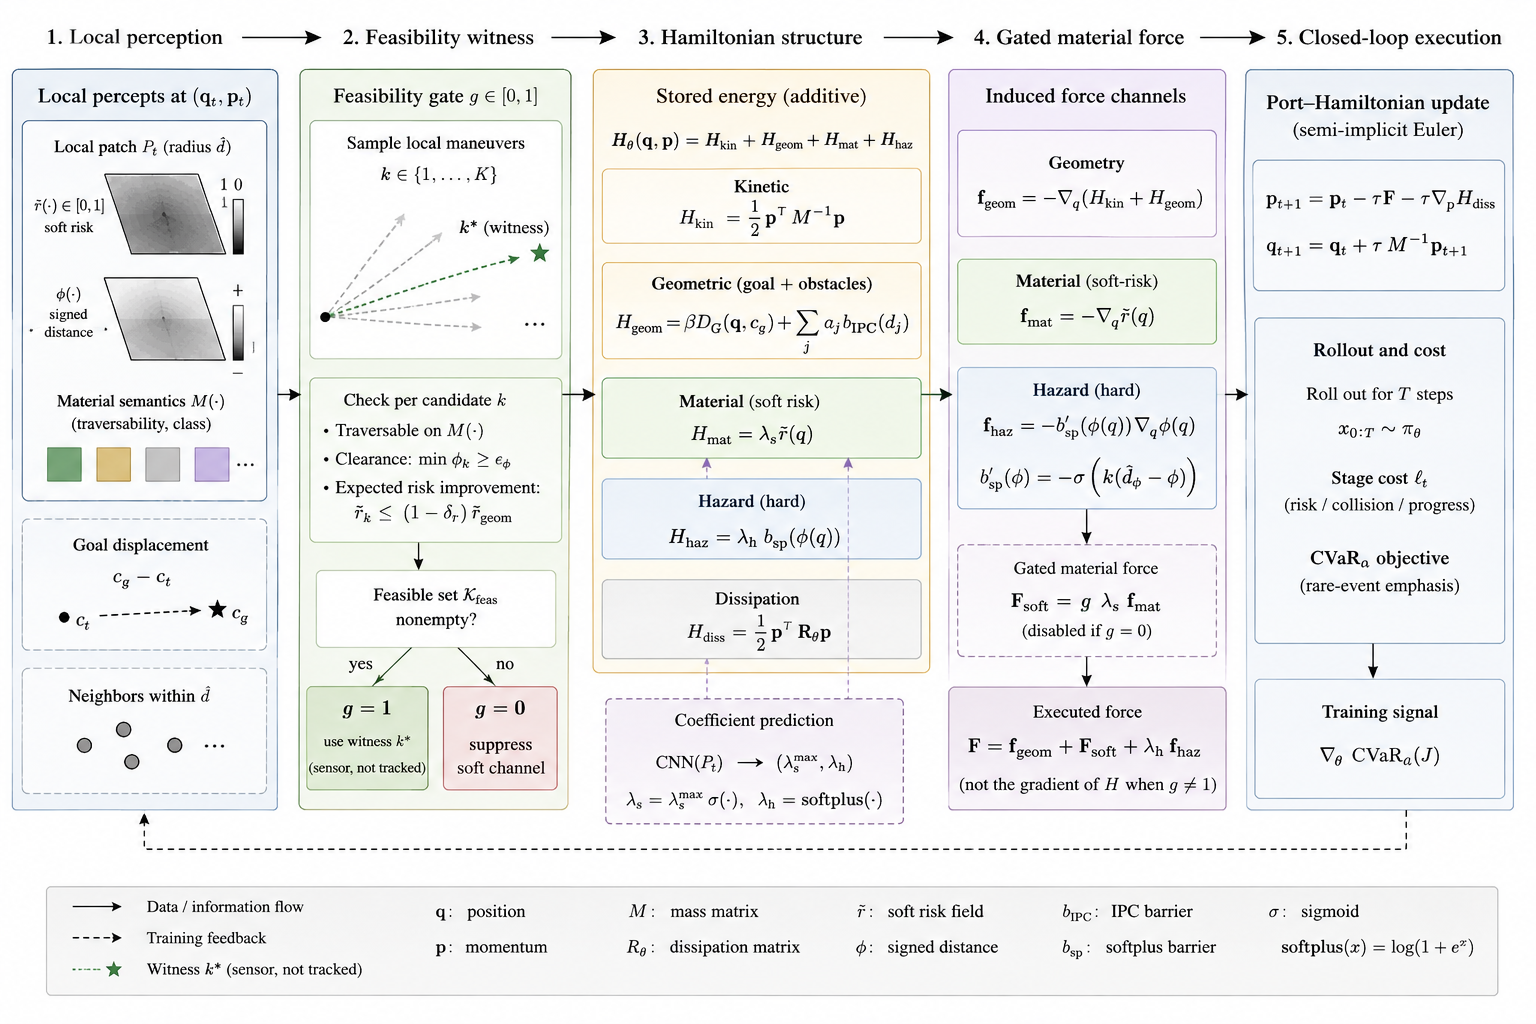
\includegraphics[width=\textwidth]{figures/overview_pipeline.png}
% \caption{{\color{red} Yi: change it to vector graphics or high res image. First column preferred to be code visualized results.} \textbf{Material-aware port-Hamiltonian navigator.} A local patch (soft risk $\tilde r$, SDF $\phi$, traversability, goal) sets coefficients $\lambda_s,\lambda_h$ and a feasibility \emph{witness} gate $g\in[0,1]$; material risk enters as an additive energy term whose force is integrated by a shared port-Hamiltonian update and trained with a CVaR objective. The witness $k^\star$ is evidence a lower-risk motion exists, not a tracked path; the gate exposes only the material channel ($\mathbf F=\mathbf f_{\rm geom}+g\,\lambda_s\mathbf f_{\rm mat}+\lambda_h\mathbf f_{\rm haz}$, not the gradient of $H$ when $g\ne1$; $g{=}0$ recovers the geometry-only field).}
% \label{fig:teaser}
% \label{fig:witness_gate}
% \end{figure*}

\subsection{Tail-sensitive training and execution}
\label{sec:method:cvar}

Each rollout accumulates a cost combining goal error, path length, soft-risk exposure, and hazard contact,
\begin{equation}
J(\theta) =
w_g\|\Pos_T-\Pos_g\|^2
+ w_\ell\!\sum_t\|\Pos_{t+1}-\Pos_t\|
+ w_r\!\sum_t\tilde r(\Pos_t)\|\Pos_{t+1}-\Pos_t\|
+ w_h\!\sum_t\mathbf{1}[\phi(\Pos_t)<\epsilon].
\label{eq:method:J}
\end{equation}
Because the consequential failures are rare, we train the coefficient heads on the empirical Rockafellar-Uryasev CVaR of $J$~\citep{rockafellar2000optimization} rather than its mean. The training objective is
\begin{equation}
\widehat{\cvar{\alpha}}(\theta)
=
\hat\eta
+\frac{1}{(1-\alpha)B}\sum_{i=1}^{B}\bigl(J^{(i)}(\theta)-\hat\eta\bigr)_+,
\qquad
\hat\eta=\widehat Q_\alpha(\{J^{(i)}\})\ \text{detached},
\label{eq:method:cvar_emp}
\end{equation}
with $\alpha=0.95$, $B=64$, so gradient concentrates on the worst rollouts~\citep{hong2014monte}. CVaR is the tail-sensitive optimizer for the learned coefficients; it does not itself decide feasibility and does not guarantee activation or suppression.

\paragraph{Offline vs.\ online.} \emph{Offline}, we load the geometry-only checkpoint with $\lambda_s,\lambda_h\equiv0$ (so Eq.~\eqref{eq:method:exec} initially reproduces the geometry-only field), then train the risk encoder and coefficient heads by backpropagating Eq.~\eqref{eq:method:cvar_emp} through the differentiable rollout, with a curriculum that advances only after validation violations fall below a threshold. \emph{Online}, each control step reads the patch, predicts $(\lambda_s,\lambda_h)$, builds $F_{\rm mat}$ and $F_{\rm haz}$, samples the $K$ witnesses, evaluates $g$, forms $F$ by Eq.~\eqref{eq:method:exec}, and integrates Eq.~\eqref{eq:method:skeleton}. No global planner is called at any step; "zero-replan" refers to this absence of global replanning. An inherited segment corrector may additionally refine the \emph{geometric} coefficients from realized local residuals at deployment; it touches neither the material channel nor the gate, and full details are in Appendix. For the logged $500$-epoch highway runs the geometry-only policy trained $1.49$\,h and the material-aware policy $3.27$\,h on one A100 ($4.8$ GPU-hours total).

\subsection{Properties and scope}
\label{sec:method:props}

We separate what follows from the material force channel from what follows from the gate, and state both as finite-horizon predictions rather than certificates.

\begin{proposition}[Material-channel and gate properties]
\label{prop:enrichment}
Let the material-aware and geometry-only policies share the geometric Hamiltonian, dissipative port $R_\theta$, mass matrix $\Mass$, and integrator, and let $F_{\rm mat}=\lambda_s f_{\rm mat}$ with the gate $g$ of Eq.~\eqref{eq:method:gate}. Under the boundedness and local-Lipschitz assumptions of Appendix~\ref{app:theory}, over any finite horizon, the following three statements hold.
\begin{enumerate}
  \item[\textbf{C1.}] \emph{Geometry-only preservation (force).} If $\sup_t\|g_t\lambda_s f_{\rm mat}(q_t)\|\le\varepsilon$ in particular if $\lambda_s\!\to\!0$ or $g\!\to\!0$ the material-aware rollout stays within $O(\varepsilon)$ of the geometry-only rollout.
  \item[\textbf{C2.}] \emph{Bounded lateral deviation under suppressed force (gate).} If $\sup_t\|P_\perp\,g_t\lambda_s f_{\rm mat}(q_t)\|\le \varepsilon_\perp$, lateral deviation from the geometry-only rollout is bounded by $O(\varepsilon_\perp)$. In particular, when the gate suppresses ($g\!\to\!0$) because no witness passes, the exposed lateral force is small and so is the induced lateral motion.
  \item[\textbf{C3.}] \emph{Selective risk descent (force).} If a feasible lateral direction has projected risk-gradient margin $\Delta$ and hard-barrier forces cancel the soft force by at most $\chi$, then when the gate admits ($g\!\approx\!1$), $\|P_\perp F_{\rm mat}\|\ge\lambda_s\Delta-\chi$ and one semi-implicit step decreases local soft risk by $O(\tau^2\lambda_s\Delta^2)$ whenever $\lambda_s\Delta>\chi$.
\end{enumerate}
\end{proposition}

C1 and C3 are properties of the force channel; C2 is a property of the gated exposure. C3 makes the effect scale with $\lambda_s$, which the experiments confirm across regimes. On dense semantic maps $\lambda_s$ is large and the isolated soft channel measurably lowers soft risk (consistent with C3, Sec.~\ref{sec:exp_dfc}), whereas on sparse off-road maps $\lambda_s$ is small and its isolated effect is near zero (Table~\ref{tab:one_factor}). Table~\ref{tab:main_theory_checks} maps each statement to the rollout condition that tests it.

\begin{table}[t]
\centering
\caption{\textbf{Main-text checks of the predictions}, as finite-rollout
statistics rather than certificates. Each row names the rollout condition under
which the prediction is testable and the statistic measured there. C1
(preservation) and C2 (suppression) concern the gated exposure, while C3 concerns
risk descent once the force is admitted. C1 is drawn from
Table~\ref{tab:delayed_escape}, C2 from
App.~Table~\ref{tab:app_rellis_full}, and C3 from Table~\ref{tab:one_factor}.
A passing statistic is evidence consistent with the prediction on these
rollouts, not a guarantee; the formal statements and their assumptions are in
App.~\ref{app:theory}.}
\label{tab:main_theory_checks}
\small
\setlength{\tabcolsep}{4pt}
\renewcommand{\arraystretch}{1.06}
\begin{tabular}{llc}
\toprule
Prediction & Rollout condition & Measured \\
\midrule
C1 (preservation) & geometry-only, delayed escape & false pre-act $0.000$ \\
C2 (suppression)  & gate off / no witness, blocked R2 & FAR $0.114$ \\
C3 (risk descent) & material force admitted, DFC ($\lambda_s$ large) & soft risk $10.340\!\to\!10.288$ \\
\bottomrule
\end{tabular}
\end{table}